\chapter{Contents of CD}

In the main directory of the cd, there is a \texttt{cmake} source for
compilation of the application.

\paragraph{Directory \texttt{/doc/thesis}}

Contains \LaTeX\ sources with \texttt{Makefile} for the compilation of
this thesis.

\paragraph{Directory \texttt{/examples}}

Contains examples written in \textsc{MONA} syntax for deciding. Ranging from
simple examples used for testing functionality to more complex ones used for
evaluation of the created code.

\paragraph{Directory \texttt{/include/vata}}

Contains headers needed to be included during the compilation of program for
part of the functions that are used from the \texttt{libvata} library.

\paragraph{Directory \texttt{/src/app/DecisionProcedure}}

Contains main part of the application sources that does the conversion of given
representation of formulae into the non-deterministic automaton and the
procedure for deciding validity or satisfiability.

\paragraph{Directory \texttt{/src/app/Frontend}}

Contains part of the sources that does the parsing of the input formulae
specification into inner representation in program

\paragraph{Directory \texttt{/src/libs}}

Contains external libraries that are used in application. Namely these are
several libraries needed for \textsc{MONA} frontend and the \texttt{libvata}
library for manipulating with NTA.

\chapter{WS$k$S specification syntax}\label{syntax}

The following grammar describes supported subset of \textsc{MONA} syntax
for the specification of verified formulae. It uses the classical BNF-like
notation.
For full syntax for \textsc{MONA} program consult the tool manual \cite{monamanual}.

\subsubsection{Specification}
\begin{verbatim}
program ::= (header;)? (declaration;)+
header ::=  ws1s | ws2s
\end{verbatim}

\subsubsection{Declarations}
% TODO: Not complete
\begin{verbatim}
declaration ::= formula
             |  var0 (varname)+
             |  var1 (varname)+
             |  var2 (varname)+
             |  'pred' varname (params)? = formula
             |  'macro' varname (params)? = formula
\end{verbatim}

\subsubsection{Formulae}
\begin{verbatim}
formula ::= 'true' | 'false' | (formula)
         |  zero-order-var
         | ~formula
         | formula | formula
         | formula & formula
         | formula => formula
         | formula <=> formula
         | first-order-term = first-order-term 
         | first-order-term ~= first-order-term 
         | first-order-term < first-order-term 
         | first-order-term > first-order-term
         | first-order-term <= first-order-term 
         | first-order-term >= first-order-term
         | second-order-term = second-order-term
         | second-order-term = { (int)+ }
         | second-order-term ~= second-order-term
         | second-order-term 'sub' second-order-term
         | first-order-term 'in' second-order-term
         | ex1 (varname)+ : formula
         | all1 (varname)+ : formula
         | ex2 (varname)+ : formula
         | all2 (varname)+ : formula
\end{verbatim}

\subsubsection{First-order terms in WS1S}
\begin{verbatim}
first-order-term ::= varname | (first-order-term)
                  |  int
                  | first-order-term + int
\end{verbatim}

\subsubsection{Second-order terms in WS1S}
\begin{verbatim}
second-order-term ::= varname | (second-order-term)
                   |  second-order-term + int
\end{verbatim}

\chapter{Usage}
The usage of the decision procedure tool is:
\begin{center}
 \texttt{dWiNA [options] <filename>}
\end{center}
\texttt{<filename>} is relative or absolute path to specification of WS$k$S
formula as defined by syntax described in Appendix \ref{syntax}. The options
that can be further set are following:
\begin{itemize}
  \item[\texttt{-t}],\texttt{--time}\,--\,prints elapsed time for decision
  procedure and further information about timing of procedure.
  \item[\texttt{-d}],\texttt{--dump-all}\,--\,dumps information about AST
  representation of given formula, symbol table, created automaton and etc.
  \item[\texttt{-q}],\texttt{--quiet}\,--\,suppress printing of information
  about decision process.
  \item[]\texttt{--reorder-bdd}\,--\,by default variables are reorder according
  to the prefix of the given formula. This can be suppressed by adding parameter
  \texttt{no} or random reordering can be done by option \texttt{random}.
\end{itemize}

\section{Instalation}

To compile the application run the following command from the main directory:

\begin{verbatim}
  $ make release
\end{verbatim}

\noindent To run the application use the following command or consult the usage:
\begin{verbatim}
  $ ./dWiNA ./examples/formulae/in.mona
\end{verbatim}

\chapter{List of Atomic Formulae}

We list in this Appendix automata corresponding to atomic formulae of WS$k$S
logic used in decision procedure. These automata are further used for
the construction of initial base automaton as described in Section \ref{wsks}.
This appendinx is structured into two parts: first describes the basic set of
atomic formulae defined for restricted syntax (see \ref{restricted}) and the other
lists automata for the extension of syntax we are supporting to optimize size of
used automata.

Note that all shown automata are non-deterministic and we use symbol
$\overline{X}$ as a substitute for any symbol of $\Sigma$, i.e. we do not care
about its value.

\section{Atomic formulae for restricted syntax}

\begin{figure}[h!]
 \begin{center}
  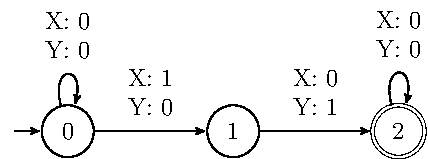
\includegraphics{fig/atomic-equal-succ}
 \end{center}
 \caption{Automaton corresponding to atomic formulae $X = Y1$, i.e. $Y$ is
 successor of $X$.}
\end{figure}

\begin{figure}[h!]
 \begin{center}
  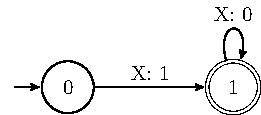
\includegraphics{fig/atomic-equals-zero}
 \end{center}
 \caption{Automaton corresponding to atomic formulae $X = \epsilon$.}
\end{figure}

\begin{figure}[h!]
 \begin{center}
  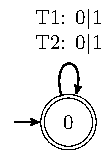
\includegraphics{fig/atomic-equal-terms}
 \end{center}
 \caption{Automaton corresponding to atomic formulae $T_1 = T_2$, where $T_1$
 and $T_2$ are two second-order variables.}
\end{figure}

\begin{figure}[h!]
 \begin{center}
  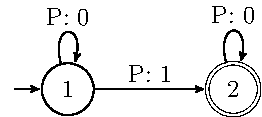
\includegraphics{fig/atomic-singleton}
 \end{center}
 \caption{Automaton corresponding to atomic formulae $\mathit{Singleton}(P)$,
 i.e. that $P$ is set containing exactly one element.}
\end{figure}

\begin{figure}[h!]
 \begin{center}
  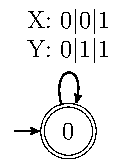
\includegraphics{fig/atomic-subset}
 \end{center}
 \caption{Automaton corresponding to atomic formulae $X \subseteq Y$}
\end{figure}
\newpage
\section{Extending restricted syntax}

\begin{figure}[h!]
 \begin{center}
  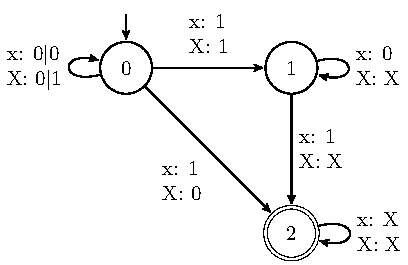
\includegraphics{fig/atomic-x-in-X}
 \end{center}
 \caption{Automaton corresponding to atomic formulae $x \in X$}
\end{figure}

\begin{figure}[h!]
 \begin{center}
  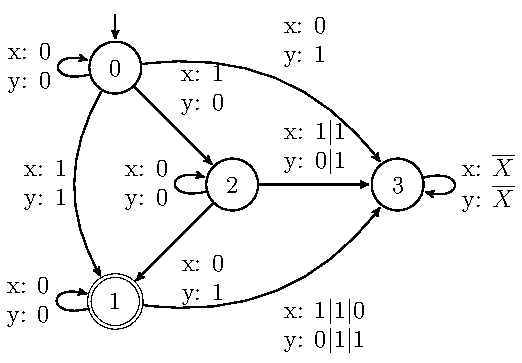
\includegraphics{fig/atomic-x-lesseq-y}
 \end{center}
 \caption{Automaton corresponding to atomic formulae $x \leq y$}
\end{figure}

\begin{figure}[h!]
 \begin{center}
  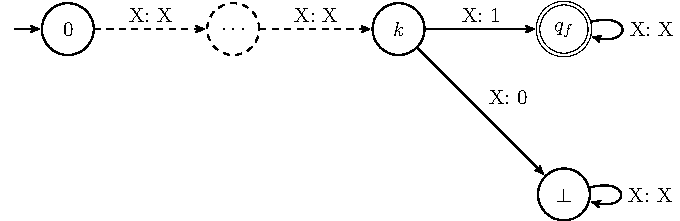
\includegraphics{fig/atomic-konst-in-X}
 \end{center}
 \caption{Automaton corresponding to atomic formulae $\mathtt{const} k \in X$}
\end{figure}

\begin{figure}[h!]
 \begin{center}
  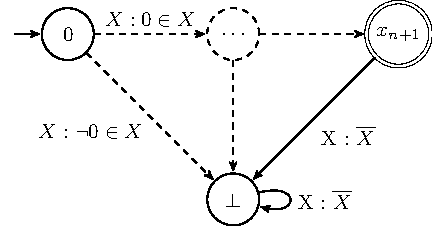
\includegraphics{fig/atomic-set-is-X}
 \end{center}
 \caption{Automaton corresponding to atomic formulae $X = \{x_1,\ldots,x_n\}$,
 for some ordering of integer constants $x_1 \leq \ldots \leq x_n$.}
\end{figure}

%\chapter{Konfigra�n� soubor}
%\chapter{RelaxNG Sch�ma konfigura�n�ho soboru}
%\chapter{Plakat}

